\section*{Digital Timing}
Digital timing algorithm uses directly the digitized waveforms, performing a digital signal treatment similar to the analog one.
 
The CFD method works generating a bipolar signal from the original pulse and then computing its zero crossing as time reference. Lets name $W_t$ the digitized waveform with $t$ an integer number (sample number). The bipolar pulse $P_t$ is calculated as:
\begin{equation}
P_t=\chi W_t-W_{t-\delta},
\label{eq:bipolarCFD}
\end{equation}
where $\chi$ is a reduction fraction and $\delta$ an integer delay.  Fig.~\ref{Fig:DigitalCFD} shows the CFD method applied on a signal. 
\begin{figure}[h!]
	\centering
	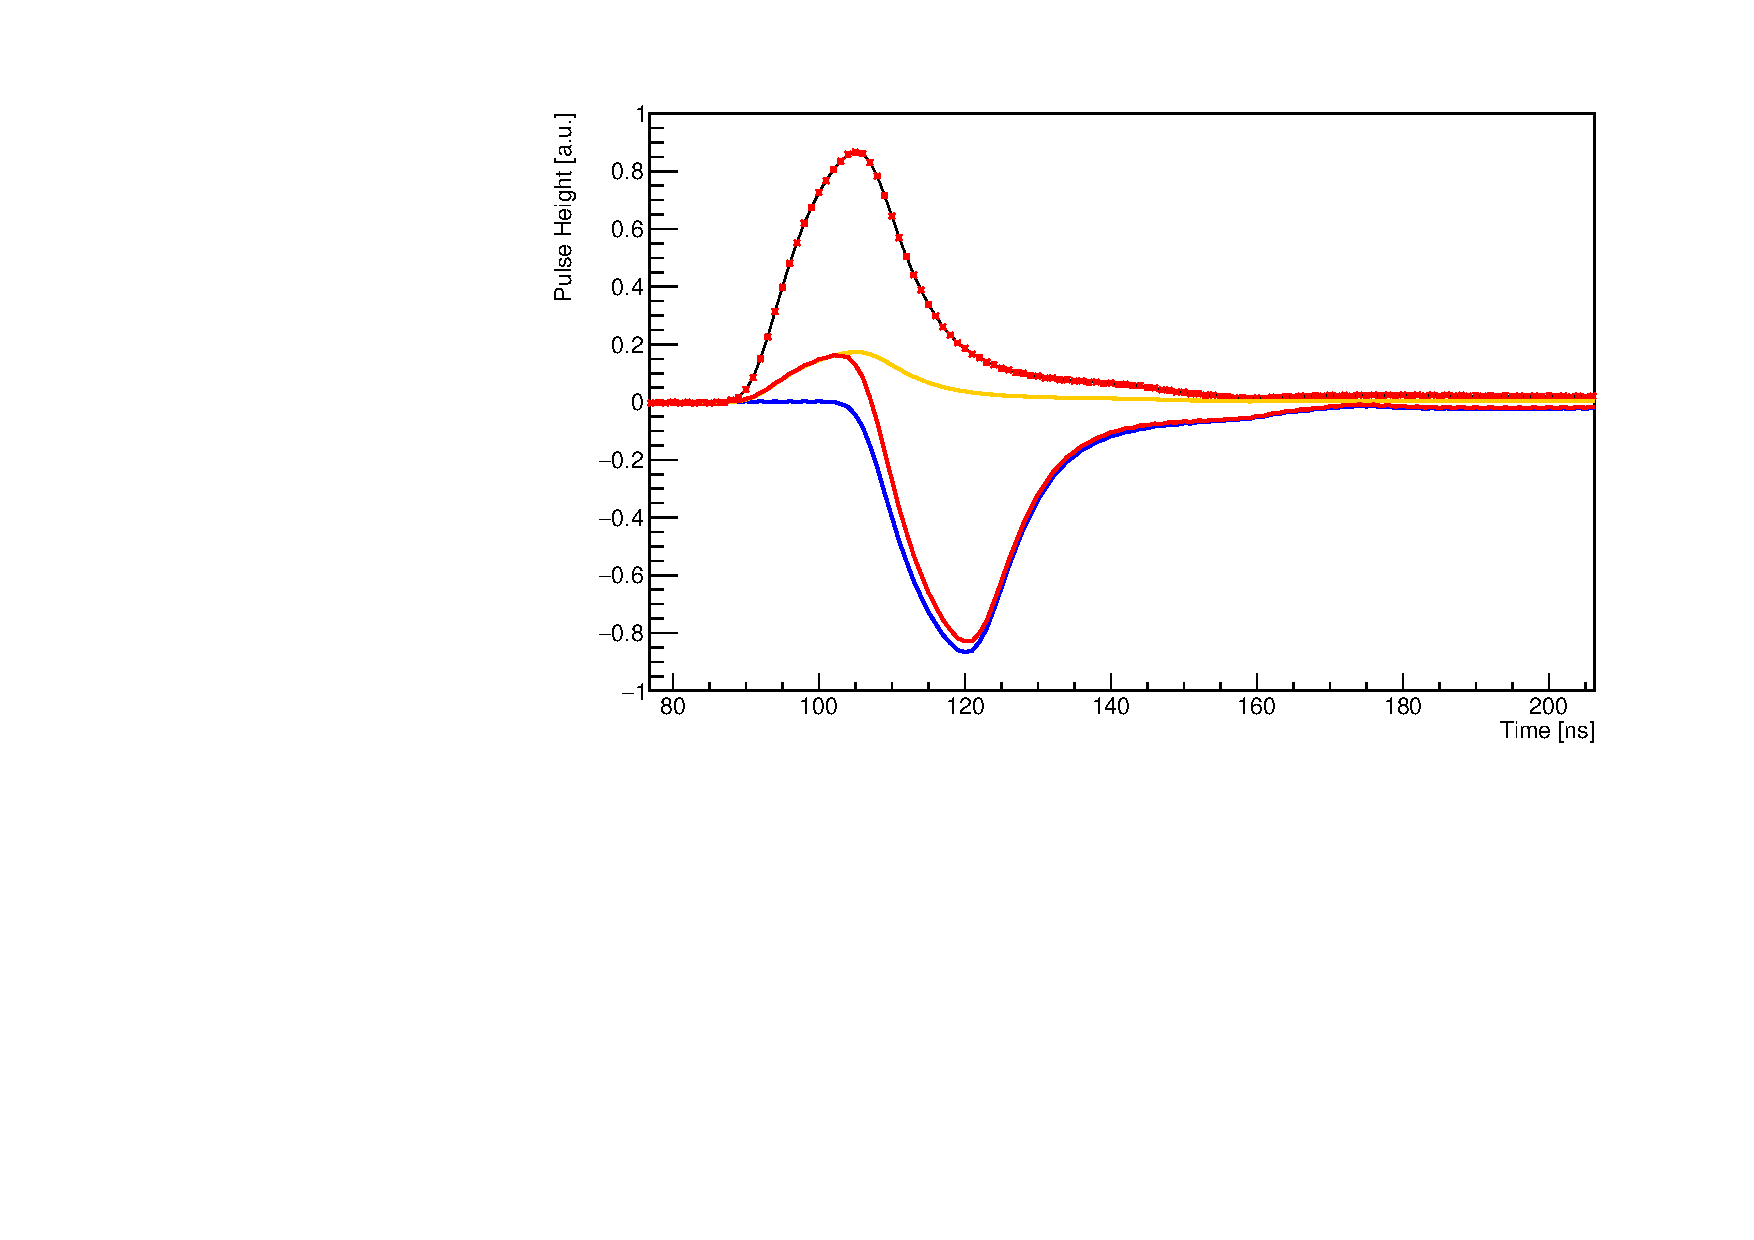
\includegraphics[width=\textwidth]{AverageCFD}
	\caption{Digital waveform obtained as average of $10^3$ normalized signals. The Delayed and fractioned signals with their sum are represented too. }
	\label{Fig:DigitalCFD}
\end{figure}

The intersection with the axis is found by taking the samples above and below  it  and interpolating to find the time reference. 
A cubic spline interpolation with derivative bound continuity condition up to second order was chosen.
Lets consider the sample range $[t_{-1},t_{0}]$ with $t_{0}$ the first sampled point after the intersection and $t_{-1}$ the preceding one. The reconstructed pulse $f(t)$ inside the range is evaluated as follow:\\
\[\mathbf{f(t)=a (t-t_{-1})^3+b (t-t_{-1})^2+c (t-t_{-1})+d}\]
\[
\left\{
\begin{aligned}
a &=1/18 (P_{t_{-3}}-8 P_{t_{-2}}+19 P_{t_{-1}}-19 P_{t_{0}}+8 P_{t_{1}}-P_{t_{2}})\\
b &=1/30 (-4 P_{t_{-3}}+32 P_{t_{-2}}-58 P_{t_{-1}}+37 P_{t_{0}}-8 P_{t_{1}}+ P_{t_{2}})\\
c &=1/90 (7 P_{t_{-3}}-56 P_{t_{-2}}-11 P_{t_{-1}}+74 P_{t_{0}}-16 P_{t_{1}}+2 P_{t_{2}})\\
d &=P_{t_{-1}}
\end{aligned}
\right.
\]


